\documentclass[11pt]{beamer}
% \documentclass[10pt]{beamer}

% \usetheme{Pittsburgh}
\usetheme{metropolis}
% \usetheme{Hannover}
% \usetheme{AnnArbor}
% \usetheme{Bergen}
% \usetheme{Berkeley}
% \usetheme{Frankfurt}
% \usetheme{Warsaw}

% \usecolortheme{owl} % dark theme
% \usecolortheme[snowy]{owl} % black on white
\usecolortheme[cautious]{owl}% dark wo redef colors

\usepackage{appendixnumberbeamer}
\usepackage[T1]{fontenc}
\usepackage[utf8]{inputenc}
% \usepackage{lmodern}
\usepackage{tikz}  

\usepackage{booktabs}
\usepackage[scale=2]{ccicons}

\usepackage{pgfplots}
\usepgfplotslibrary{dateplot}

\usepackage{xspace}
\usepackage{tabularx}

\newcommand{\themename}{\textbf{\textsc{metropolis}}\xspace}

\title{ Hoot revenue strategy : video AR ads using CPR model}
\subtitle{Performant AR ads with measurable ROI - making video ads perform using AR call-to-actions plus CPR model}
\date{\today}
\author{Hoot AR ads team}
\institute{Hoot Live inc., a Delaware C-corp}
% \titlegraphic{\hfill
\includegraphics[height=1.5cm]{logo.pdf}}

\begin{document}
\maketitle

% \begin{frame}{Table of contents}
%  \setbeamertemplate{section in toc}[sections numbered]
%  \tableofcontents[hideallsubsections]
% \end{frame}

% \section{Primer}

\begin{frame}[fragile]{Current landscape in digital video advertising}
	% \begin{itemize}%needs pause
 % \setbeamercovered{transparent}%show dimmed
 % \begin{itemize}[<+->]%uncover piecewise
 \begin{itemize}[<+-| alert@+>]%uncover w highlight 
	 
\item[-]current video advertising biz model is based on ROI blind CPM (cost per million impressions) pricing model
 % \pause
\item[-]which does not provide an accurate ROI picture for advertisement buyers
 % \pause
\item[-]Many ad-bots end up generating fake video ad views creating uncertainty/ speculation about the actual cost, effectiveness \& ROI of the ad
% \pause
\item[-]ad pageview or impression is an obsolete metric lacking accountability of relevance, effectiveness \& performance 
\item[-]CPM model based on impressions earns lower revenue as there is no ROI \& users are flooded with more irrelevant video ads that do not convert
\end{itemize}

\end{frame}
\begin{frame}[t]{Problems of current CPM video ad model}
\begin{enumerate}[<+-| alert@+>]
\item No clear call to actions in current video ads
% \pause
\item Viewers are confused as to what to do after watching video
% \pause
\item advertisers still pay unnecessary \$ for ad bot \& fake social-media video views
% \pause
\item Viewers are not engaged enough in the video ad leading to significant drop in engagement \& subsequently sales for advertisers
% \pause
\item viewers do not buy the product they are forced to view on an irrelevant video ad
\item leading to unclear ROI to advertisers top-line/bottomline

\end{enumerate}
\pause
Video ads are still stuck in the  dark ages reminiscent of banner ad days pre-Google Adwords

\end{frame}
\begin{frame}[t]{Augmented Reality has its iPhone/Netscape moment}
 \begin{itemize}[<+-| alert@+>]
	\item[=]Apple 🍎
	 iOS ARKit \& Google 🤖 Android ARCore are bringing AR tech to the masses at scale
	% \pause
	\item[=]Pokemon Go is an early indicator of market readiness \& consumer adoption of AR tech
	% \pause
	\item[=]Timing is just right for AR ads
	% \pause
	\item[=]Total Addressable market is \$ 60-100 Billion USD 
	% \pause
	\item[=]Unprecedented market opportunity as 600(100 android + 500 iOS) million smartphones are going to be AR ready by Q1 2018
\end{itemize}
\end{frame}
%--- Next Frame ---%
\begin{frame}[t]{Hoot Augmented Reality ads 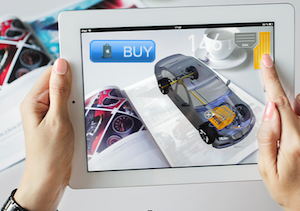
\includegraphics[scale=.1]{static/arad/arad5}} 
 \begin{itemize}[<+-| alert@+>]
\item[*]interactive AR models feel less like spammy ads \& more like engaging content leading to increased viewer engagement \& virality 
% Content \& Virality: 
% \pause	
\item[*]Augmented reality ads create great engagement with users in key ways
% \pause
\item[*]Personalization: users \& celebrities can upload bitmoji ar avatars to become part of the ad
% \pause

\includegraphics[scale=.15]{static/arad/bitmoji} 
% (masquerade)
% \pause
\item[*]so celebrities like Rihanna can help engagement by using her avatar in an AR ad \& help make it more viral 
% \pause
\item[*]with clear \underline{Calls to action} "Buy now" buttons can be programmatically added to the ad, e.g., \emph{ Buy concert ticket to Rihanna event}
\end{itemize}
\end{frame}
%--- Next Frame ---%
% Big hairy audacious goal

\begin{frame}[fragile]{BHAG Solution - Building Adwords of video 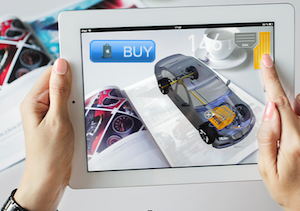
\includegraphics[scale=.1]{static/arad/arad5} }
\begin{itemize}[<+-| alert@+>]
\item Interactive AR models increase viewer engagement
% \pause	
\item Clear, useful \& engaging call to actions in video ads using AR after diving user-intent
% \pause
\item Viewers \underline{know} what action to take after watching video ad by clicking call to action buy 
% \pause
\item Clear AR ad performance \textsc{ROI} to advertisers 
% \pause
\item show more relevant ads with higher conversions less frequently than CPM video ads leading to a quantifiably superior user experience 
% \pause
\end{itemize}
\pause
Relevant \textsc{Hoot AR ads} helps usher a golden age of performant video ads like Google did to banner ads through Adwords


\end{frame}

\begin{frame}[t]{Hoot CPR model - video Adwords economics}
\begin{itemize}[<+-| alert@+>]
\item[*] Hoot AR ads uses a CPR model powered by a \textsc{Vickrey} auction engine
% \pause
\item[*]\emph{A Vickrey auction is one in which the winner pays the second-highest price, not the price they themselves bid}
% \pause
\item[*]which allows Hoot to monetize only if the consumer clicks through to advertisers call to action
% \pause
\item[*]and price based on a \textsc{CPR(cost per referral)} model which is not based on ineffectively measuring impressions
\item[*]making this model ROI aware \& fake impression resistant
\item[*]This benefits advertisers as they can now see clear ROI picture for their ad-spend dollars \$
\end{itemize}
\end{frame}


\begin{frame}[t]{Hoot CPR model - video Adwords economics}
\begin{itemize}[<+-| alert@+>]

\item[*]Buy actions are completed using irreversible \textsc{Bitcoin ETH} cryptocurrency txns instead of tedious credit cards further reducing friction \& fraud
% \pause
\item[*]Google Adwords \& Amazon proved Conversions \& Referrals > pageviews \& eyeballs in keyword advertising \& e-commerce respectively
\item[*]we want to bring this to the video ad world by ushering in CPR based performance pricing model
% \pause
\item[*]This benefits hoot as we can now price based on measurable effectiveness as Google was able to charge significantly more for Adwords based on performance laying foundations for a multi-billion dollar ad biz

\end{itemize}
\end{frame}
\begin{frame}[standout]
 Hoot AR ads Questions? - building Adwords of the web
 \begin{tikzpicture}
 \node (img1) {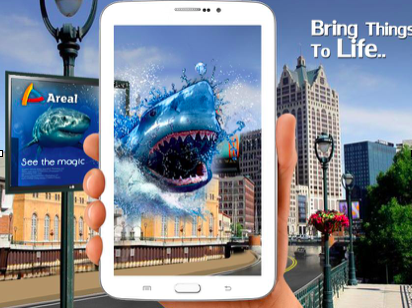
\includegraphics[height=5cm]{static/arad/arad1}};
 % \pause
 \node (img2) at (img1.south east) [xshift=-1cm] {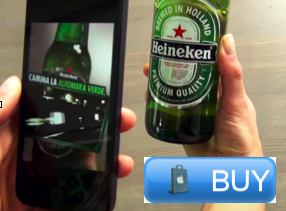
\includegraphics[height=4cm]{static/arad/arad3}};
 % \pause
 \node (img3) at (img2.south west) [xshift=-2cm,yshift=1cm] {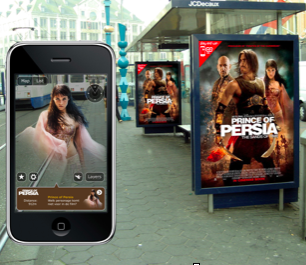
\includegraphics[height=4cm]{static/arad/arad2}};
 \pause
 \node (img4) {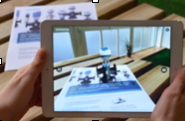
\includegraphics[height=2cm]{static/arad/arad4}};
 % \pause
 \node (img5) at (img1.south east) [yshift=-1cm] {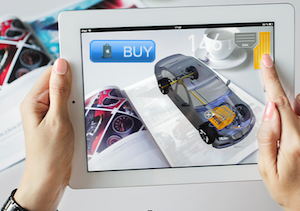
\includegraphics[height=4cm]{static/arad/arad5}};
 
 \end{tikzpicture}
 
\end{frame}

 % \section{Description}

\begin{frame}[allowframebreaks,fragile]{Hoot Performant AR video ads + measurable ROI = Building Adwords of video}
\begin{footnotesize}%
	Video Ads have been priced historically based on CPM for impressions as it has been nearly impossible to know how much of these video ads lead to a product sale/conversion or if they even positively affect the customer ROI. Viewers do not know what action to take and how to take the said action leaving them to figure out how to follow up on the video ad they just saw, leading to a lot of drop off and lack of performance of these video ads. Hence It’s not easy  to measure effectiveness and performance of the video ads historically.

Using interactive \textbf{Hoot AR} augmented reality  ads with clear
call to actions such as a buy button or rent button below the
interactive Hoot AR ad, sales can be generated right then and there,
after the viewer interacts with the Hoot AR ad. We will be able to
charge based on sales generated from the AR interaction i.e.,
referrals and instead of pricing based on CPM or impressions we can
price based on  cost per referral(\textbf{CPR}). The CPR price becomes
the signal that drives the continuous auction engine that powers the
Hoot ad marketplace. By bringing about an innovative CPR based
business model to video ads using Augmented reality
\emph{call-to-actions} we bring the effectiveness of Google AdWords to
video ads that only used to perform as well as banner ads
before. Hence Hoot AR ads, improves the effectiveness of plain video
ads, leading to a quantum improvement in video adspend ROI much like
AdWords improved the ROI of web based banner ads, laying the
foundation for a billion dollar ads business.

\end{footnotesize}



\end{frame}


\end{document}
